\subsection*{7.4\hspace*{0.5cm}Energy with Spring - Question}
A low friction cart with a mass of 0.25kg travels along a horizontal track and collides
head on with a spring that has a spring constant of $155\frac{N}{m}$.
If the Spring was compressed by 6.0cm, how fast was the cart initially travelling?
\subsection*{7.4\hspace*{0.5cm}Energy with Spring - Graph and Givens}
\begin{minipage}{0.5\textwidth}
    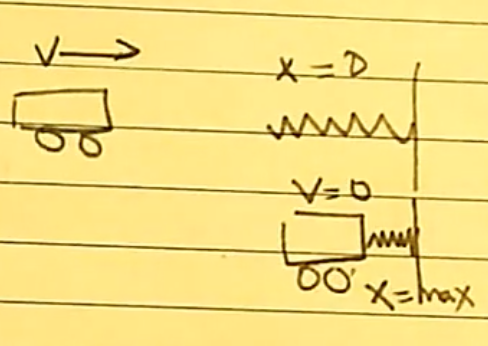
\includegraphics[scale=0.33]{./images/springs.png}
\end{minipage}
\begin{minipage}{0.5\textwidth}
    \begin{itemize}
        \item $x = 6.0cm$
        \item $k = 155\frac{N}{m}$
        \item $m_{c} = 0.25kg$
        \item $v_{c} = ?$
    \end{itemize}
\end{minipage}
\subsection*{7.4\hspace*{0.5cm}Energy with Spring - Solve}
Because the cart is not initially colliding with the spring, $E_{e}$ is zero. Because the cart's velocity post-collision is zero, $E_{k}\prime$ is also zero. Because the cart and the spring are at the same height both before and after the collision, both $E_{g}$ and $E_{g}\prime$ are set to zero.\newline\newline
\textbf{1.} $E_{tot} = E_{tot}\prime$ \\
\begin{adjustwidth}{0.6cm}{0pt}
    $E_{k} + \cancelto{0}{E_{g}} + \cancelto{0}{E_{e}} = \cancelto{0}{E_{k}\prime} + \cancelto{0}{E_{g}\prime} + E_{e}\prime$ \\\\
    $E_{k} = E_{e}\prime$ \\\\
    $\frac{1}{2}m_{c}v_{c}^2 = \frac{1}{2}kx^2$ \\\\
    $\therefore v_{c} = \sqrt[]{\frac{kx^2}{m_{c}}} = \sqrt[]{\frac{(155){(6.0)}^2}{(0.25)}} \approx 149\frac{m}{s}$
\end{adjustwidth}\vspace*{15pt}
\textbf{2.} $h_{c} = 9.2m$ \\
\begin{adjustwidth}{0.6cm}{0pt}
    $E_{k} + E_{g} + \cancelto{0}{E_{e}} = \cancelto{0}{E_{k}\prime} + \cancelto{0}{E_{g}\prime} + E_{e}\prime$ \\\\
    $E_{k} + E_{g} = E_{e}\prime$ \\\\
    $\frac{1}{2}m_{c}v_{c}^2 + m_{c}gh = \frac{1}{2}kx^2$ \\\\
    $\therefore v_{c} = \sqrt[]{\frac{(kx^2) - (m_{c}gh)}{m_{c}}} = \sqrt[]{\frac{(155){(6.0)}^2 - (0.25)(9.81)(9.2)}{(0.25)}} \approx 149\frac{m}{s}$
\end{adjustwidth}\vspace*{15pt}